\chapter {Conclusions}
\label{ch:con}

\section {Conclusion}

In this dissertation, we explored the physics-based probable maximum precipitation estimation using numerical models:

1. We established a numerical modeling framework based on the WRF model. For extreme precipitation simulation purpose, the combination of medium grid size (5km), Morrison microphysics scheme with Kain-Fritsch cumulus scheme can be taken as a starting point in the model calibration. Through our extended validation, this combination is often among the best model configurations that we tested. Since many atmospheric models share a common collection of parameterization schemes, this recommendation can also be applied to other models.

2. Using WRF model, we examined our capability of reconstructing extreme precipitation events of various types and locations across the US since the 1900s. We found that with currently available model input (initial/boundary conditions), only those extreme events after the 1940s can be satisfactorily constructed. Therefore, for model-based PMP estimations, the historical storms we should examine are only those after the 1940s.

3. We outlined the guidance to make a physics-based PMP estimation. Through the statistical analysis of major long-term reanalysis products (NARR and ERA-Interim), we found that the extreme precipitation in the west US is more related to extreme vertical fields, while those extreme events in the east US are more related to extreme moisture availability. Therefore, we recommend that the PMP estimation in the west US should be done through maximization of vertical wind fields, while PMP in the east US should be estimated by maximizing the moisture availability in the model input.

4. To facilitate the transition from traditional PMP estimation approach to the proposed physics-based approach, we also proposed a novel hybrid approach to bridge these approached. The motivation of this hybrid approach is illustrated in figure \ref{fig:1-1}. This helps engineering community to achieve a stepwise adoption of physics-based approach, and understand how the different input data and methods would impact the final PMP estimation. Such hybrid approach can also be used as a starting point of checking the existing infrastructures (which are designed under traditional PMPs) under the projected climate change.

5. Our proposed approaches (e.g., physics-based and hybrid methods) are able to produce ensemble PMP estimates given multiple model input, which is readily available from projects such as CMIP5. This helps to determine the uncertainty within the PMP estimation.

\section{Future work}
Through our study, we give out the recommended way to make physics-based PMP estimation. However, for these guidelines to become engineering protocol, the following works are still needed:

1. Extensive studies are required that validate these recommendations over the historical storms. This is to convince the engineering communities to confidently adopt these guidelines.

2. More details on how the model should be run with these guidelines should be investigated. For example, how the simulation boundaries should be defined (right along the watershed boundary v.s. a larger box), how the climatology of vertical wind should be defined for the various precipitation event duration (1-hour to 72-hour), as well as how to systematically set the desired initial/boundary conditions in the model simulation. Eventually, a systematic and detailed instructions are required for the engineering practice.

3. In developing the physics-based guidelines, we checked the roles of atmospheric instability, moisture availability, wind fields and temperature profiles in the extreme precipitation duration. If there are other factors that may be considered as important environmental factors in the storm duration, they should also be analyzed.

4. So far, all of the above analyses are done only for the US. With the reanalysis products available at global scale, it is possible and necessary to conduct such analysis globally. This would reveal the spatial patterns of the relationship between extreme precipitation and environmental conditions at larger scale. At the same time, such analysis is more useful for the PMP estimation in the regions where long-term ground observation has not been established. Figure \ref{fig:6-1} is such an example.

With these additional works complete, the proposed physics-based PMP estimation approach would be ready for engineering implementation. With such a full dynamic method, we can advance our engineering safety design with a more robust basis (i.e., more historical storms that can be taken from atmospheric reanalysis), as well as a more forward thinking fashion (i.e., designs under a changing climate). Also we will be ready to explore the various interactions between natural variability, human activities and engineering infrastructure safety in a more comprehensive way.

\begin{figure}[htbp]
	\centering
	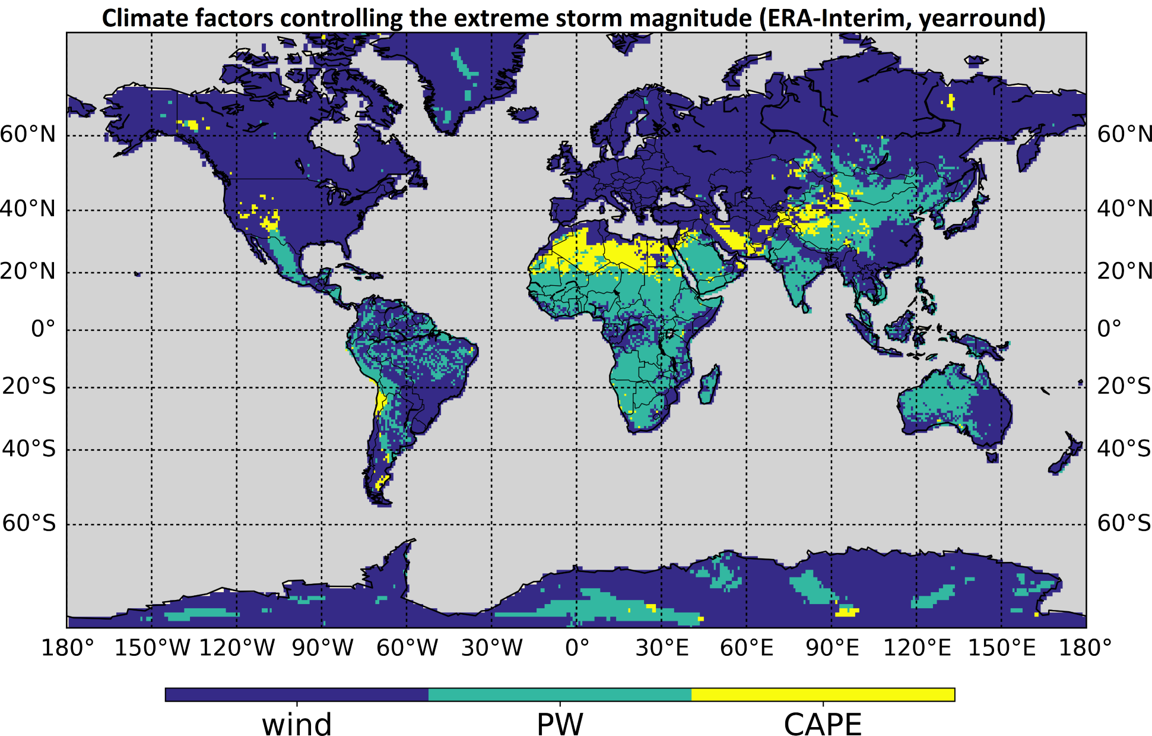
\includegraphics[width=\linewidth]{pics/ch6/fig1.png}
	\caption{A complete transition from traditional approach to physics-based approach of PMP estimation.}
	\label{fig:6-1}
\end{figure}